% !TEX root = ../../prj4projektdokumentation.tex
% SKAL STÅ I TOPPEN AF ALLE FILER FOR AT MASTER-filen KOMPILERES 

\section{Blok definitionsdiagram}
Et BDD for spændingsregulator ses på figur \ref{fig:BDDSpaendingsregulator}. På diagrammet ses de overordnet blokke spædingsregulator består af. En beskrivelse af hver blok kan læses under figur \ref{fig:BDDSpaendingsregulator}.

\begin{figure}[htbp] % (alternativt [H])
	\centering
	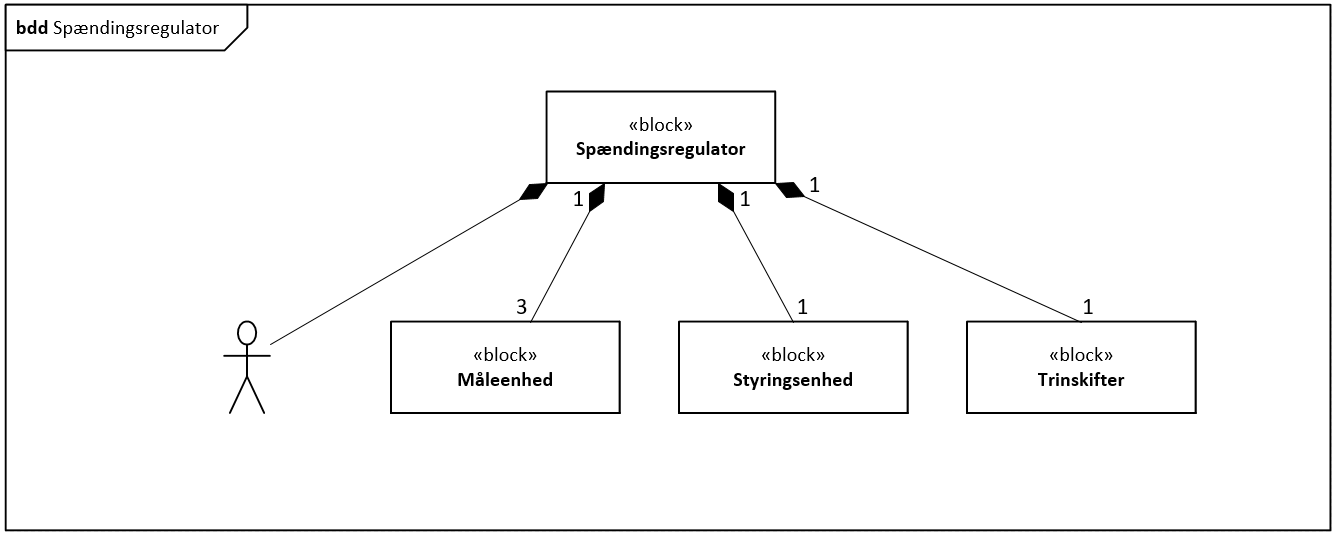
\includegraphics[width=0.9\textwidth]{Figure/BDDSpaendingsregulator}
	\caption{BDD Spændingsregulator}
	\label{fig:BDDSpaendingsregulator}
\end{figure}

\textbf{Måleenhed} står for at måle spænding, strøm og faseforskydningen herimellem. Ligeledes skal denne kunne måle indeholdet af harmoniske frekvenser. Den består af hardware til måling af de nævnte parametre og en PSoC 5. På enheden ligger også en del af behandlingen af rådataet, så dette kan formidles til styringsenheden.

\textbf{Styringsenhed} har til opgave at styre trinskifteren ud fra de data den får fra målenehderne. Den består af en PLC, tl styringen og et HMI, der skal give en bruger overblik over status for distributionslinjen.

\textbf{Trinskifter} er en enhed der kan skifte trin på transformeren ud fra et signal fra styringsenheden. Den består altå af en kontakt for hvert trin, der kan kontrolleres af styringsenheden.